\section{Contexte, données à traiter et objectif}
\begin{frame}{Contexte, données à traiter et objectif}
Compétition Casp
\begin{center}
\footnotesize
\begin{tabular}{ccc}
    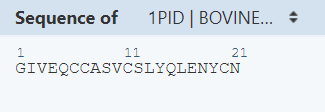
\includegraphics[width=3cm]{sequence_insuline_bovine}
    & 
    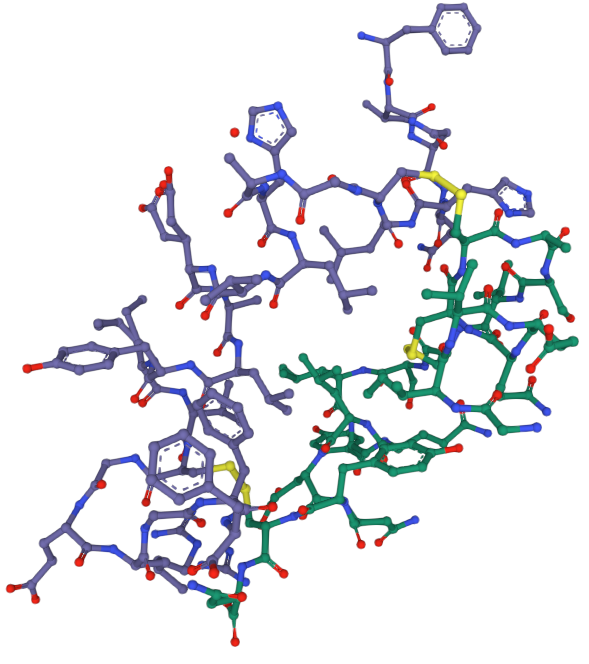
\includegraphics[width=2cm]{structure_insuline_bovine}
    &
    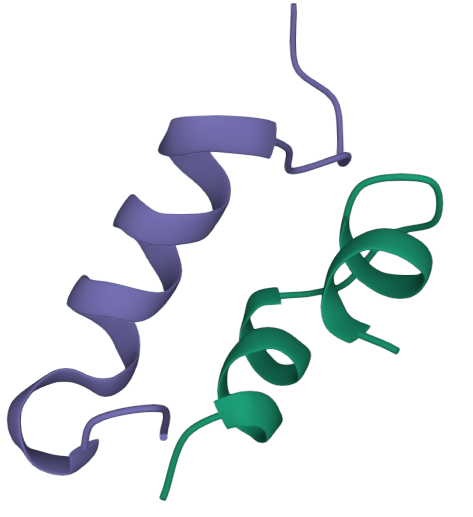
\includegraphics[width=2cm]{cartoon_insuline_bovine} \\
    \textit{Séquence} & \textit{Structure} & \textit{Représentation simplifiée}
\end{tabular}
\newline \newline \underline{ex} : protéine d'insuline bovine 
\footnote{source : Protein Data Bank, https://www.rcsb.org/3d-view/1B0Q}
\end{center}
\small
\underline{Objectif} : proposer une méthode de comparaison de structures
\end{frame}